\section{Aufbau}
In Abbildung \ref{fig:Aufbau} ist der Aufbau des Versuches schematisch abgebildet.
Zur Erzeugung von Spektrallinien wird eine Cadmium-Lampe in einen Elektromagneten gebracht.
Das transversal abgestrahlte Licht der Lampe wird duch eine Objektivlinse und eine Kondensorlinse auf einen Spalt kollimiert und hinter dem Spalt durch eine Line auf einen Geradsichtprisma fokussiert.
Hinter dem Prisma wird ein Polarisationsfilter zur Selektion der $\pi$ und $\sigma$ Linien und eine weitere Linse aufgebaut.
Da hinter diesen nun die einzelnen Spektrallinien zu sehen sind, kann eine dieser Linien durch einen weiteren, verschiebbaren Spalt ausgewählt werden.
Hinter dem Spalt wird die ausgewählte Spektrallinie durch eine Linse auf die Eintrittsfläche einer Lummer-Gehrcke Platte fokussiert.
Das hinter der Lummer-Gehrcke Platte erzeugte Interferenzmuster kann mit einer Digitalkamera aufgenommen und analysiert werden.

\begin{figure}[H]
  \centering
  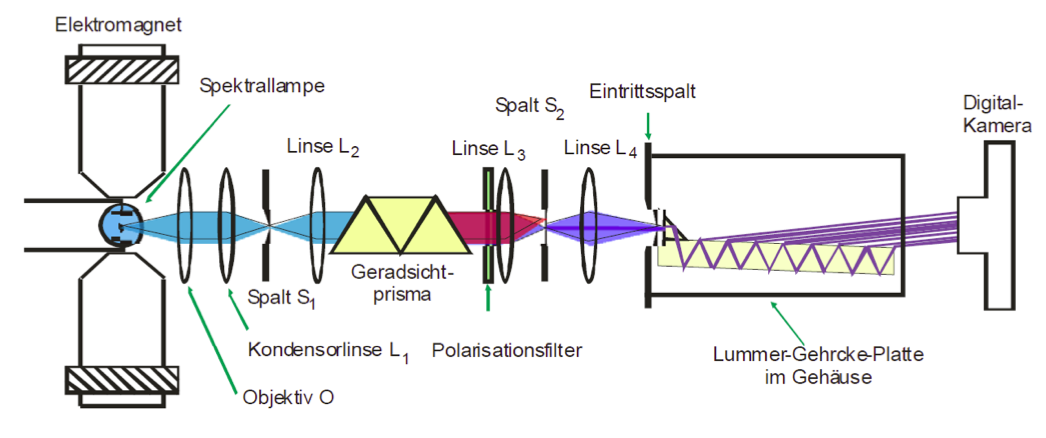
\includegraphics[width = .7\textwidth]{images/Aufbau.png}
  \caption{Schematische Darstellung des Versuchsaufbaus \cite{Anleitung}.}
  \label{fig:Aufbau}
\end{figure}

\subsection{Lummer-Gehrcke Platte}

Eine Lummer-Gehrcke Platte funktioniert wie ein hochauflösendes Spektrometer mit einem sehr kleinen Auflösungsbereich.
Diese bestehlt aus einer planparallelen Glasplatte, das eingestrahlte Licht wird an der Oberseite der Platte reflektiert und gebrochen.
Somit kommt es auf der Länge $L$ der Platte an vielen Stellen zu gebrochenen Lichtstrahlen, welche miteinander interferieren.
Eine Abbildung einer Lummer-Gehrcke Platte ist in Abbildung \ref{fig:Lummer-Gehrcke} dargestellt.
\par\medskip
Durch eine Veränderung $\Delta \lambda$ der eingestrahlten Wellenlänge durch eine Veränderung des Magnetfeldes, kommt es zu Verschiebung $\delta s$ der Interferenzstreifen.
Damit es nicht zur Überlagerung der Streifen kommt, darf die Aufspaltung nicht größer sein als
\begin{equation*}
  \Delta \lambda = \frac{\lambda^2}{2d} \frac{1}{\sqrt{n^2-1}} \, .
\end{equation*}

Um diese Grenze nicht zu überschreiten, muss das Magnetfeld in Abgängigkeit der Energieaufspaltung und damit der Landé-Faktoren $g_J$ eingestellt werden.
Für die maximale Magnetfeldstärke folgt
\begin{equation} \label{eqn:B}
  B = \frac{\Delta \lambda}{4} \frac{h c}{\lambda} \frac{1}{\mu_B g_J} \,.
\end{equation}
Die Magnetfeldstärke muss also vor Versuchdurchführung für die vermuteten Landé-Faktoren eingestellt werden.
